\documentclass{standalone}
\usepackage{tikz}
\usetikzlibrary{patterns, positioning}


\begin{document}
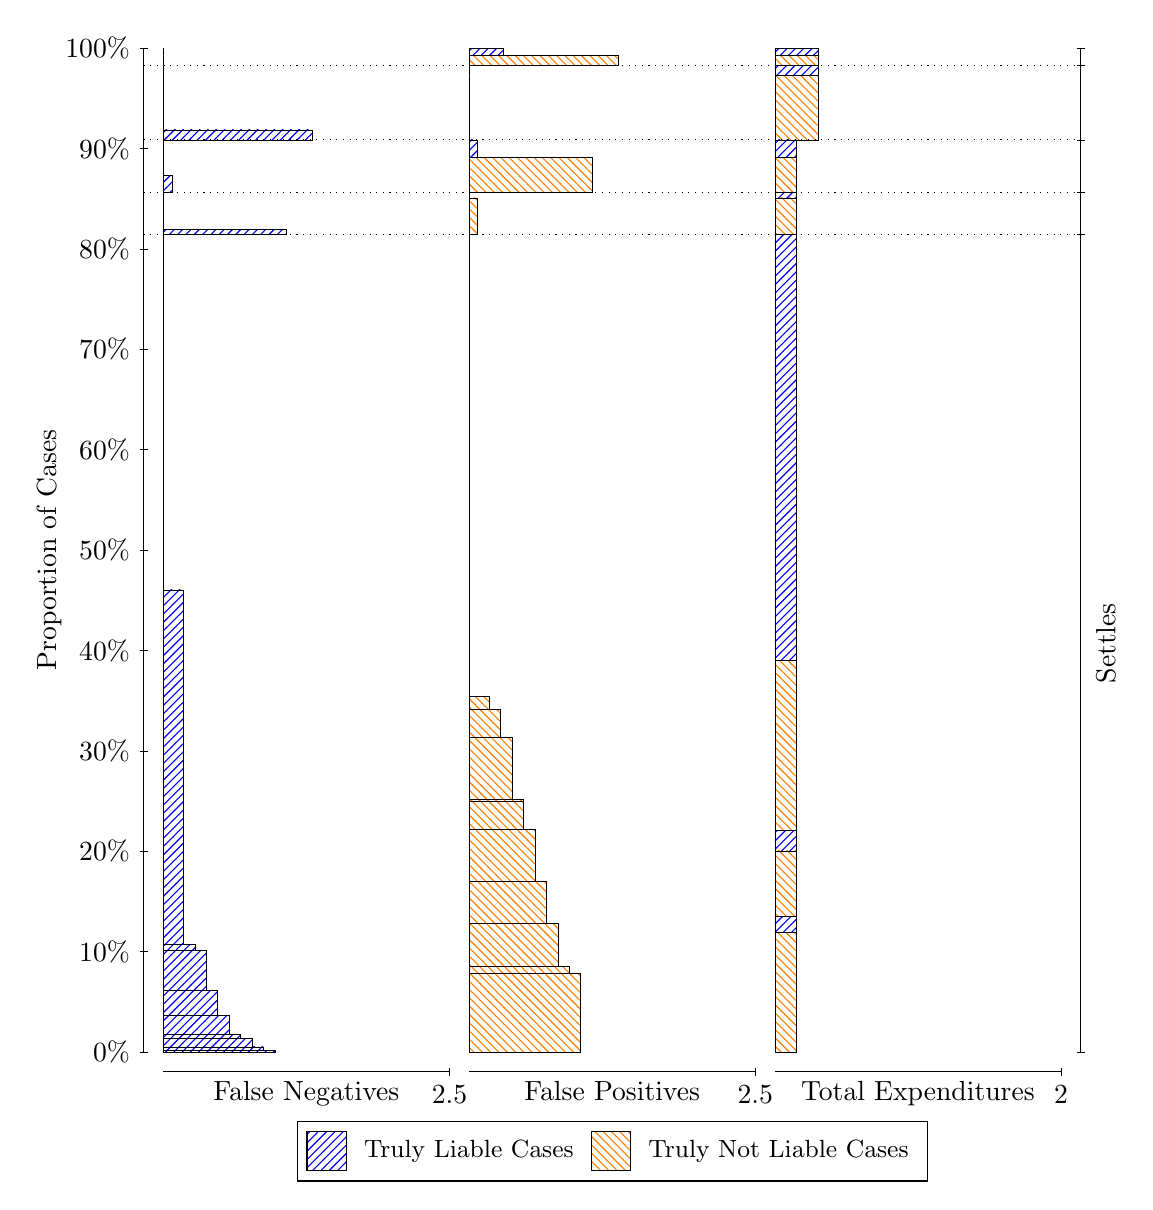
\begin{tikzpicture}
\draw[black, very thin] (1.5,1.75) -- (1.5,14.5);
\node[rotate=90, text=black, anchor=center] at (0.3, 8.125) {Proportion of Cases};
\draw[black, very thin] (1.45,1.75) -- (1.55,1.75);
\node[text=black, anchor=east] at (1.45, 1.75) {0\%};
\draw[black, very thin] (1.45,3.025) -- (1.55,3.025);
\node[text=black, anchor=east] at (1.45, 3.025) {10\%};
\draw[black, very thin] (1.45,4.3) -- (1.55,4.3);
\node[text=black, anchor=east] at (1.45, 4.3) {20\%};
\draw[black, very thin] (1.45,5.575) -- (1.55,5.575);
\node[text=black, anchor=east] at (1.45, 5.575) {30\%};
\draw[black, very thin] (1.45,6.85) -- (1.55,6.85);
\node[text=black, anchor=east] at (1.45, 6.85) {40\%};
\draw[black, very thin] (1.45,8.125) -- (1.55,8.125);
\node[text=black, anchor=east] at (1.45, 8.125) {50\%};
\draw[black, very thin] (1.45,9.4) -- (1.55,9.4);
\node[text=black, anchor=east] at (1.45, 9.4) {60\%};
\draw[black, very thin] (1.45,10.675) -- (1.55,10.675);
\node[text=black, anchor=east] at (1.45, 10.675) {70\%};
\draw[black, very thin] (1.45,11.95) -- (1.55,11.95);
\node[text=black, anchor=east] at (1.45, 11.95) {80\%};
\draw[black, very thin] (1.45,13.225) -- (1.55,13.225);
\node[text=black, anchor=east] at (1.45, 13.225) {90\%};
\draw[black, very thin] (1.45,14.5) -- (1.55,14.5);
\node[text=black, anchor=east] at (1.45, 14.5) {100\%};

\draw[black, very thin] (13.4,1.75) -- (13.4,14.5);
\draw[black, very thin] (13.35,1.75) -- (13.45,1.75);
\node[anchor=west] at (13.35, 1.75) {};
\draw[black, very thin] (13.35,12.132) -- (13.45,12.132);
\node[anchor=west] at (13.35, 12.132) {};
\draw[black, very thin] (13.35,12.662) -- (13.45,12.662);
\node[anchor=west] at (13.35, 12.662) {};
\draw[black, very thin] (13.35,13.334) -- (13.45,13.334);
\node[anchor=west] at (13.35, 13.334) {};
\draw[black, very thin] (13.35,14.279) -- (13.45,14.279);
\node[anchor=west] at (13.35, 14.279) {};
\draw[black, very thin] (13.35,14.5) -- (13.45,14.5);
\node[anchor=west] at (13.35, 14.5) {};

\draw[black, very thin, pattern color=blue, pattern=north east lines] (1.75,1.75) rectangle (3.167,1.7692);
\draw[black, very thin, pattern color=blue, pattern=north east lines] (1.75,1.7692) rectangle (3.0217,1.8153);
\draw[black, very thin, pattern color=blue, pattern=north east lines] (1.75,1.8153) rectangle (2.8763,1.9203);
\draw[black, very thin, pattern color=blue, pattern=north east lines] (1.75,1.9203) rectangle (2.731,1.9719);
\draw[black, very thin, pattern color=blue, pattern=north east lines] (1.75,1.9719) rectangle (2.5857,2.2103);
\draw[black, very thin, pattern color=blue, pattern=north east lines] (1.75,2.2103) rectangle (2.4403,2.5342);
\draw[black, very thin, pattern color=blue, pattern=north east lines] (1.75,2.5342) rectangle (2.295,3.042);
\draw[black, very thin, pattern color=blue, pattern=north east lines] (1.75,3.042) rectangle (2.1497,3.1164);
\draw[black, very thin, pattern color=blue, pattern=north east lines] (1.75,3.1164) rectangle (2.0043,7.618);
\draw[black, very thin, pattern color=orange, pattern=north west lines] (1.75,7.618) rectangle (1.75,12.132);
\draw[black, very thin, pattern color=blue, pattern=north east lines] (1.75,12.132) rectangle (3.3123,12.196);
\draw[black, very thin, pattern color=orange, pattern=north west lines] (1.75,12.196) rectangle (1.75,12.662);
\draw[black, very thin, pattern color=blue, pattern=north east lines] (1.75,12.662) rectangle (1.859,12.88);
\draw[black, very thin, pattern color=orange, pattern=north west lines] (1.75,12.88) rectangle (1.75,13.334);
\draw[black, very thin, pattern color=blue, pattern=north east lines] (1.75,13.334) rectangle (3.6393,13.461);
\draw[black, very thin, pattern color=orange, pattern=north west lines] (1.75,13.461) rectangle (1.75,14.279);
\draw[black, very thin, pattern color=orange, pattern=north west lines] (1.75,14.279) rectangle (1.75,14.402);
\draw[black, very thin, pattern color=blue, pattern=north east lines] (1.75,14.402) rectangle (1.75,14.5);
\draw[black, very thin, pattern color=orange, pattern=north west lines] (5.6333,1.75) rectangle (7.0503,2.7516);
\draw[black, very thin, pattern color=orange, pattern=north west lines] (5.6333,2.7516) rectangle (6.905,2.8348);
\draw[black, very thin, pattern color=orange, pattern=north west lines] (5.6333,2.8348) rectangle (6.7597,3.3797);
\draw[black, very thin, pattern color=orange, pattern=north west lines] (5.6333,3.3797) rectangle (6.6143,3.9116);
\draw[black, very thin, pattern color=orange, pattern=north west lines] (5.6333,3.9116) rectangle (6.469,4.5777);
\draw[black, very thin, pattern color=orange, pattern=north west lines] (5.6333,4.5777) rectangle (6.3237,4.9395);
\draw[black, very thin, pattern color=orange, pattern=north west lines] (5.6333,4.9395) rectangle (6.3237,4.9612);
\draw[black, very thin, pattern color=orange, pattern=north west lines] (5.6333,4.9612) rectangle (6.1783,5.7469);
\draw[black, very thin, pattern color=orange, pattern=north west lines] (5.6333,5.7469) rectangle (6.033,6.1012);
\draw[black, very thin, pattern color=orange, pattern=north west lines] (5.6333,6.1012) rectangle (5.8877,6.2638);
\draw[black, very thin, pattern color=blue, pattern=north east lines] (5.6333,6.2638) rectangle (5.6333,12.132);
\draw[black, very thin, pattern color=orange, pattern=north west lines] (5.6333,12.132) rectangle (5.7423,12.598);
\draw[black, very thin, pattern color=blue, pattern=north east lines] (5.6333,12.598) rectangle (5.6333,12.662);
\draw[black, very thin, pattern color=orange, pattern=north west lines] (5.6333,12.662) rectangle (7.1957,13.116);
\draw[black, very thin, pattern color=blue, pattern=north east lines] (5.6333,13.116) rectangle (5.7423,13.334);
\draw[black, very thin, pattern color=orange, pattern=north west lines] (5.6333,13.334) rectangle (5.6333,14.153);
\draw[black, very thin, pattern color=blue, pattern=north east lines] (5.6333,14.153) rectangle (5.6333,14.279);
\draw[black, very thin, pattern color=orange, pattern=north west lines] (5.6333,14.279) rectangle (7.5227,14.402);
\draw[black, very thin, pattern color=blue, pattern=north east lines] (5.6333,14.402) rectangle (6.0693,14.5);
\draw[black, very thin, pattern color=orange, pattern=north west lines] (9.5167,1.75) rectangle (9.7892,3.2735);
\draw[black, very thin, pattern color=blue, pattern=north east lines] (9.5167,3.2735) rectangle (9.7892,3.4761);
\draw[black, very thin, pattern color=orange, pattern=north west lines] (9.5167,3.4761) rectangle (9.7892,4.3049);
\draw[black, very thin, pattern color=blue, pattern=north east lines] (9.5167,4.3049) rectangle (9.7892,4.5625);
\draw[black, very thin, pattern color=orange, pattern=north west lines] (9.5167,4.5625) rectangle (9.7892,6.7241);
\draw[black, very thin, pattern color=blue, pattern=north east lines] (9.5167,6.7241) rectangle (9.7892,12.132);
\draw[black, very thin, pattern color=orange, pattern=north west lines] (9.5167,12.132) rectangle (9.7892,12.598);
\draw[black, very thin, pattern color=blue, pattern=north east lines] (9.5167,12.598) rectangle (9.7892,12.662);
\draw[black, very thin, pattern color=orange, pattern=north west lines] (9.5167,12.662) rectangle (9.7892,13.116);
\draw[black, very thin, pattern color=blue, pattern=north east lines] (9.5167,13.116) rectangle (9.7892,13.334);
\draw[black, very thin, pattern color=orange, pattern=north west lines] (9.5167,13.334) rectangle (10.062,14.153);
\draw[black, very thin, pattern color=blue, pattern=north east lines] (9.5167,14.153) rectangle (10.062,14.279);
\draw[black, very thin, pattern color=orange, pattern=north west lines] (9.5167,14.279) rectangle (10.062,14.402);
\draw[black, very thin, pattern color=blue, pattern=north east lines] (9.5167,14.402) rectangle (10.062,14.5);
\draw[black, dotted] (1.5,12.132) -- (13.4,12.132);
\draw[black, dotted] (1.5,12.662) -- (13.4,12.662);
\draw[black, dotted] (1.5,13.334) -- (13.4,13.334);
\draw[black, dotted] (1.5,14.279) -- (13.4,14.279);
\draw[black, very thin] (1.75,1.5) -- (5.3833,1.5);
\node[text=black, anchor=north] at (3.5667, 1.5) {False Negatives};
\draw[black, very thin] (5.3833,1.45) -- (5.3833,1.55);
\node[text=black, anchor=north] at (5.3833, 1.45) {2.5};

\draw[black, very thin] (5.6333,1.5) -- (9.2667,1.5);
\node[text=black, anchor=north] at (7.45, 1.5) {False Positives};
\draw[black, very thin] (9.2667,1.45) -- (9.2667,1.55);
\node[text=black, anchor=north] at (9.2667, 1.45) {2.5};

\draw[black, very thin] (9.5167,1.5) -- (13.15,1.5);
\node[text=black, anchor=north] at (11.333, 1.5) {Total Expenditures};
\draw[black, very thin] (13.15,1.45) -- (13.15,1.55);
\node[text=black, anchor=north] at (13.15, 1.45) {2};

\node[text=black, centered, rotate=90] at (13.72, 6.9409) {Settles};





\draw (7.449999999999999,1.5) node[draw=none] (baseCoordinate) {};
\begin{scope}[align=center]
        \matrix[scale=0.5, draw=black, below=0.5cm of baseCoordinate, nodes={draw}, column sep=0.1cm]{
            \node[rectangle, draw, minimum width=0.5cm, minimum height=0.5cm, pattern color=blue, pattern=north east lines] {}; &
            \node[draw=none, font=\small, text=black] (B) {Truly Liable Cases}; &
            \node[rectangle, draw, minimum width=0.5cm, minimum height=0.5cm, pattern color=orange, pattern=north west lines] {}; &
            \node[draw=none, font=\small, text=black] (B) {Truly Not Liable Cases}; \\
            };
\end{scope}

\end{tikzpicture}
\end{document}